% 2008 年北京卷理科第 12 题：折线 ABC，A(0,4)、B(2,0)、C(6,4)。
% 来源 PDF：gaokaomath-src/普通高考/2008/2008北京理.pdf
% SHA-256：1ba43840bfc822e6bcd4a1c04e69becd857890f1abf3da09910b4f26ae25c9a8
% 原页：2008北京理.pdf 第 1 页（A3 三栏）第 2 栏，书页码 425。
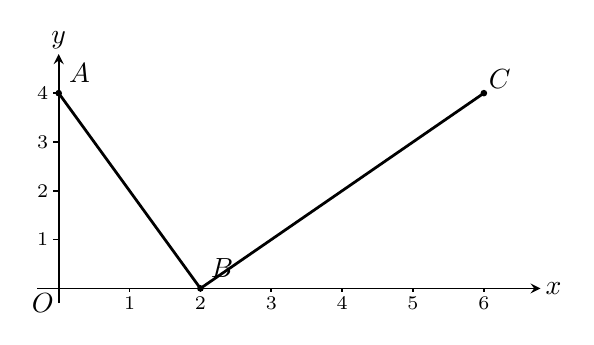
\begin{tikzpicture}[x=0.9cm, y=0.62cm, semithick,
  every node/.style={inner sep=1.5pt}]
  \draw[->,>=stealth] (-0.3,0) -- (6.8,0) node[right] {$x$};
  \draw[->,>=stealth] (0,-0.3) -- (0,4.8) node[above] {$y$};
  \node[below left] at (0,0) {$O$};
  \foreach \x in {1,2,3,4,5,6} \draw (\x,0) -- (\x,-0.08) node[below,font=\scriptsize] {$\x$};
  \foreach \y in {1,2,3,4} \draw (0,\y) -- (-0.08,\y) node[left,font=\scriptsize] {$\y$};
  \draw[line width=1pt] (0,4) -- (2,0) -- (6,4);
  \fill (0,4) circle (1.2pt) node[above right=2pt] {$A$};
  \fill (2,0) circle (1.2pt) node[above right=2pt] {$B$};
  \fill (6,4) circle (1.2pt) node[above right] {$C$};
\end{tikzpicture}
